For description of a homogeneous material, only the overall geometry of investigated region and one set of material properties are needed.
If the heterogeneities are considered, their geometry (position, shape and orientation) together with more than one set of material properties have to be specified
The material properties can be assumed as a function of position, i.e, each material point can have unique properties, or the situation may be simplified with the assumption that the properties of a material point depend only on the constituent and do not vary within the constituent.

In science and engineering, concrete is described on different scales, depending on the purpose.
In practical civil engineering, concrete is usually described as a homogeneous isotropic material.
However, for some applications, the heterogeneous internal structure of concrete plays a crucial role.

Investigated on mesoscale, concrete may be considered as a composition of continuous binder (usually hardened cement paste) matrix with inserted aggregates (such as crushed rocks, gravel or sand) and air voids (pores).

For modeling purposes, the interface transition zone (ITZ) between aggregates and matrix plays a special role.

This chapter describes the development of a discrete mesoscale model for concrete.





\chapter{State of the art}\label{chapMCPMStateOfTheArt}
Various approaches of mesoscale concrete modeling have been published.
All of them consider concrete as a matrix-based composite with aggregates as inclusions, possibly also with pores.
The approaches may be classified from several points of view.

The first significant difference is whether the model is formulated in two dimensions (see, e.g.,
\cite{%
	AzevedoLemosAlmeida2008a,%
	HafnerEckardtLutherKonke2006a,%
	WangKwanChan1999a,%
	LeiteSlowikApel2007a,%
	LeiteSlowikMihashi2004a,%
	MagnierDonze1998a,%
	PanFengJinXuSunZhangOwen2013a,%
	PedersenSimoneSluys2013a,%
	SatohYamadaIshiyama2013a,%
	WangLinGu2008a,%
	XuHaoLi2012a,%
	ZhouHao2008a,%
	ZhouHao2008b,%
	QinZhang2011a,%
	GuHongWangLin2013a,%
	GrasslJirasek2010a,%
	GrasslRempling2008a,%
	ZhuTang2002a,%
	GhoshChaudhuri2013a%
}) or in three dimensions (see, e.g.,
\cite{%
	CombypeyrotBernardBouchardBayGarciadiaz2009a,%
	LeiteSlowikApel2007a,%
	LeiteSlowikApel2007a,%
	ShahbeykHosseiniYaghoobi2011a,%
	TranDonzeMarin2011a,%
	WriggersMoftah2006,%
	KimAlrub2011a,%
	CaballeroWillamCarol2008a,%
	YipLiLiaoBolander2006a,%
	Marangi2010a,%
	Cusatis2001a,%
	CusatisBazantCedolin2006a,%
	CusatisPelessoneMencarelli2011a,%
	CusatisMencarelliPelessoneBaylot2011a,%
	Kozicki2007a,%
	LandisBolander2009a,%
	AsahinaLandisBolander2011a%
}).
Although the 3D models describe the heterogeneous geometry (apart from very special cases) more realistically, some ideas and approaches from 2D models may be useful and applicable also for the 3D case.

According to the numerical method used, the approaches can be divided into continuum and discrete based.
Although the main purpose of this work is to develop a discrete mesoscale model, continuum based approaches can be very inspiring, especially in the context of ITZ material models.
Most of the continuum based works use FEM as a numerical solution tool
\cite{%
	CombypeyrotBernardBouchardBayGarciadiaz2009a,%
	HafnerEckardtLutherKonke2006a,%
	WangKwanChan1999a,%
	LeiteSlowikApel2007a,%
	LeiteSlowikMihashi2004a,%
	OzboltSharma2012a,%
	PedersenSimoneSluys2013a,%
	SatohYamadaIshiyama2013a,%
	ShahbeykHosseiniYaghoobi2011a,%
	XuHaoLi2012a,%
	ZhouHao2008a,%
	ZhouHao2008b,%
	SnozziGatuingtMolinari2012a,%
	CaballeroWillamCarol2008a,%
	ZhuTang2002a%
}, but also other methods (meshfree methods \cite{GhoshChaudhuri2013a} or SPH method \cite{MaWangRen2011a} for instance) are used.

The discrete element method can model disintegration of materials and is therefore also very popular in the context of concrete modeling, especially for scenarios like fragmentation, impact or explosion problems etc.
How DEM is used for mesoscale concrete modeling, see, e.g.,
\cite{%
	AzevedoLemosAlmeida2008a,%
	CambordeMariottiDonze2000a,%
	GrohKonietzkyWalterHerbst2011a,%
	HentzDonzeDaudeville2004a,%
	IbrahimbegovicDelaplace2003a,%
	LambertBuzziGiacomini2010a,%
	LiuZhaoYun2011a,%
	MagnierDonze1998a,%
	PanFengJinXuSunZhangOwen2013a,%
	TranDonzeMarin2011a,%
	WangLinGu2008a,%
	QinZhang2011a,%
	GuHongWangLin2013a,%
	GrasslJirasek2010a,%
	GrasslRempling2008a,%
	YipLiLiaoBolander2006a,%
	Marangi2010a,%
	Cusatis2001a,%
	CusatisBazantCedolin2006a,%
	CusatisPelessoneMencarelli2011a,%
	CusatisMencarelliPelessoneBaylot2011a,%
	LandisBolander2009a,%
	AsahinaLandisBolander2011a%
}.

\section{Mesoscale geometry}
The concrete heterogeneous geometry (i.e, amount, sizes, shapes and orientation of aggregates and pores) plays an important role in the realistic description of concrete meso\-scale behavior.
The authors use various ways of definition of aggregate geometry, from extremely simplified regular uniformly sized hexagonal particles (see \cite{SatohYamadaIshiyama2013a} and figure \ref{figMCPMLitratureMesoGeometryExamples} top left)
through commonly used spherical/circular (see, e.g.,
\cite{%
	AzevedoLemosAlmeida2008a,%
	CombypeyrotBernardBouchardBayGarciadiaz2009a,%
	PedersenSimoneSluys2013a,%
	ShahbeykHosseiniYaghoobi2011a,%
	WangLinGu2008a,%
	WriggersMoftah2006,%
	XuHaoLi2012a,%
	ZhouHao2008a,%
	ZhouHao2008b,%
	ZhouHao2009a,%
	KimAlrub2011a,%
	GuHongWangLin2013a,%
	GrasslJirasek2010a,%
	GrasslRempling2008a,%
	YipLiLiaoBolander2006a,%
	Marangi2010a,%
	Kozicki2007a,%
	NeubauerLenningsGarboczi1996a,%
	LandisBolander2009a,%
	AsahinaLandisBolander2011a%
} and figure \ref{figMCPMLitratureMesoGeometryExamples} top middle) or ellipsoidal/elliptical (see, e.g.,
\cite{%
	GrohKonietzkyWalterHerbst2011a,%
	HafnerEckardtLutherKonke2006a,%
	LeiteSlowikApel2007a,%
	LeiteSlowikMihashi2004a,%
	SnozziGatuingtMolinari2012a,%
	KimAlrub2011a%
} and figure \ref{figMCPMLitratureMesoGeometryExamples} top right) representation to more sophisticated approximation by polygons/polyhedrons
\cite{%
	KwanWangChan1999b,%
	PanFengJinXuSunZhangOwen2013a,%
	PedersenSimoneSluys2013a,%
	KimAlrub2011a,%
	QinZhang2011a,%
	ZhuTang2002a%
} and figure \ref{figMCPMLitratureMesoGeometryExamples} bottom left,
or representation of aggregates by the series of harmonic functions
\cite{%
	Garboczi2002a,%
	HafnerEckardtLutherKonke2006a,%
	Rypl2010a%
} and figure \ref{figMCPMLitratureMesoGeometryExamples} bottom right.
\begin{figure}[ht]
	\centering
	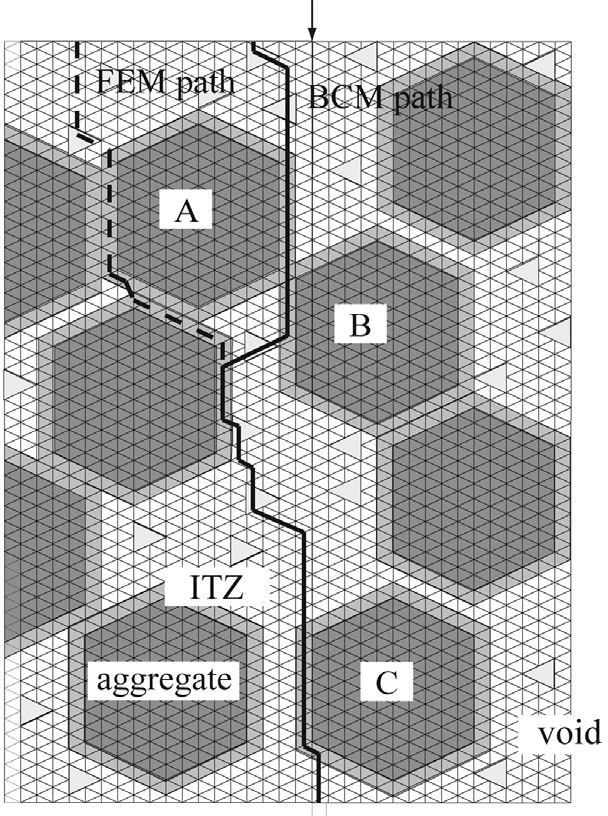
\includegraphics[height=4cm]{mcpm/geomExamples/satohEtAl}
	\hspace{10mm}
	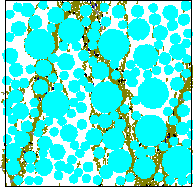
\includegraphics[height=4cm]{mcpm/geomExamples/azevedoEtAl}
	\hspace{10mm}
	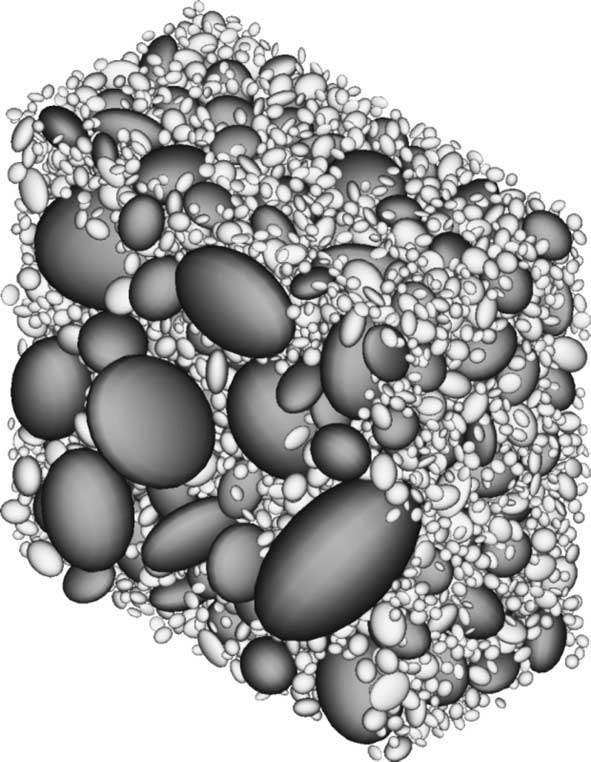
\includegraphics[height=4.5cm]{mcpm/geomExamples/hafnerEtAl}
	\par
	\vspace{2mm}
	\includegraphics[height=4cm]{mcpm/geomExamples/caballeroEtAl}
	\hspace{20mm}
	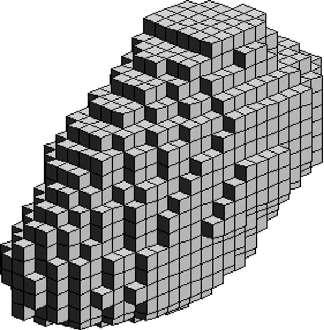
\includegraphics[height=4cm]{mcpm/geomExamples/rypl_1}
	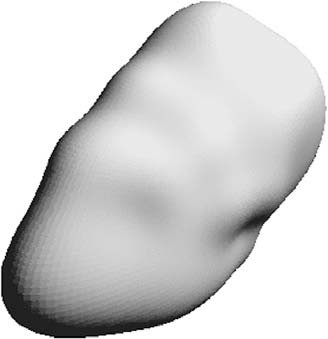
\includegraphics[height=4cm]{mcpm/geomExamples/rypl_2}
	\caption[Examples of geometrical representation of aggregates]{Examples of geometrical representation of aggregates:
		hexagonal \cite{SatohYamadaIshiyama2013a} (top left),
		circular \cite{AzevedoLemosAlmeida2008a} (top middle),
		ellipsoidal \cite{HafnerEckardtLutherKonke2006a} (top right),
		polyhedral \cite{CaballeroWillamCarol2008a} (bottom left)
		and using spherical harmonics \cite{Rypl2010a} (bottom right)
	}
	\label{figMCPMLitratureMesoGeometryExamples}
\end{figure}

For method testing and validation, there also exist experiments with artificially created mesoscale geometries, where large aggregates have predefined size, position and orientation, see
\cite{%
	TreggerCorrGrahambradyShah2006a,%
	BuyukozturkHearing1998%
} and figure \ref{figMCPMLitratureMesoGeometryArtificial}.
\begin{figure}[ht]
	\centering
	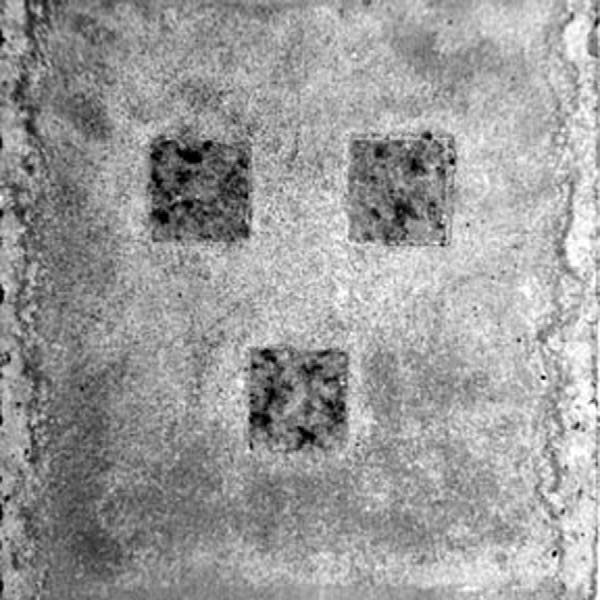
\includegraphics[width=5cm]{mcpm/geomExamples/treggerEtAl}
	\hspace{10mm}
	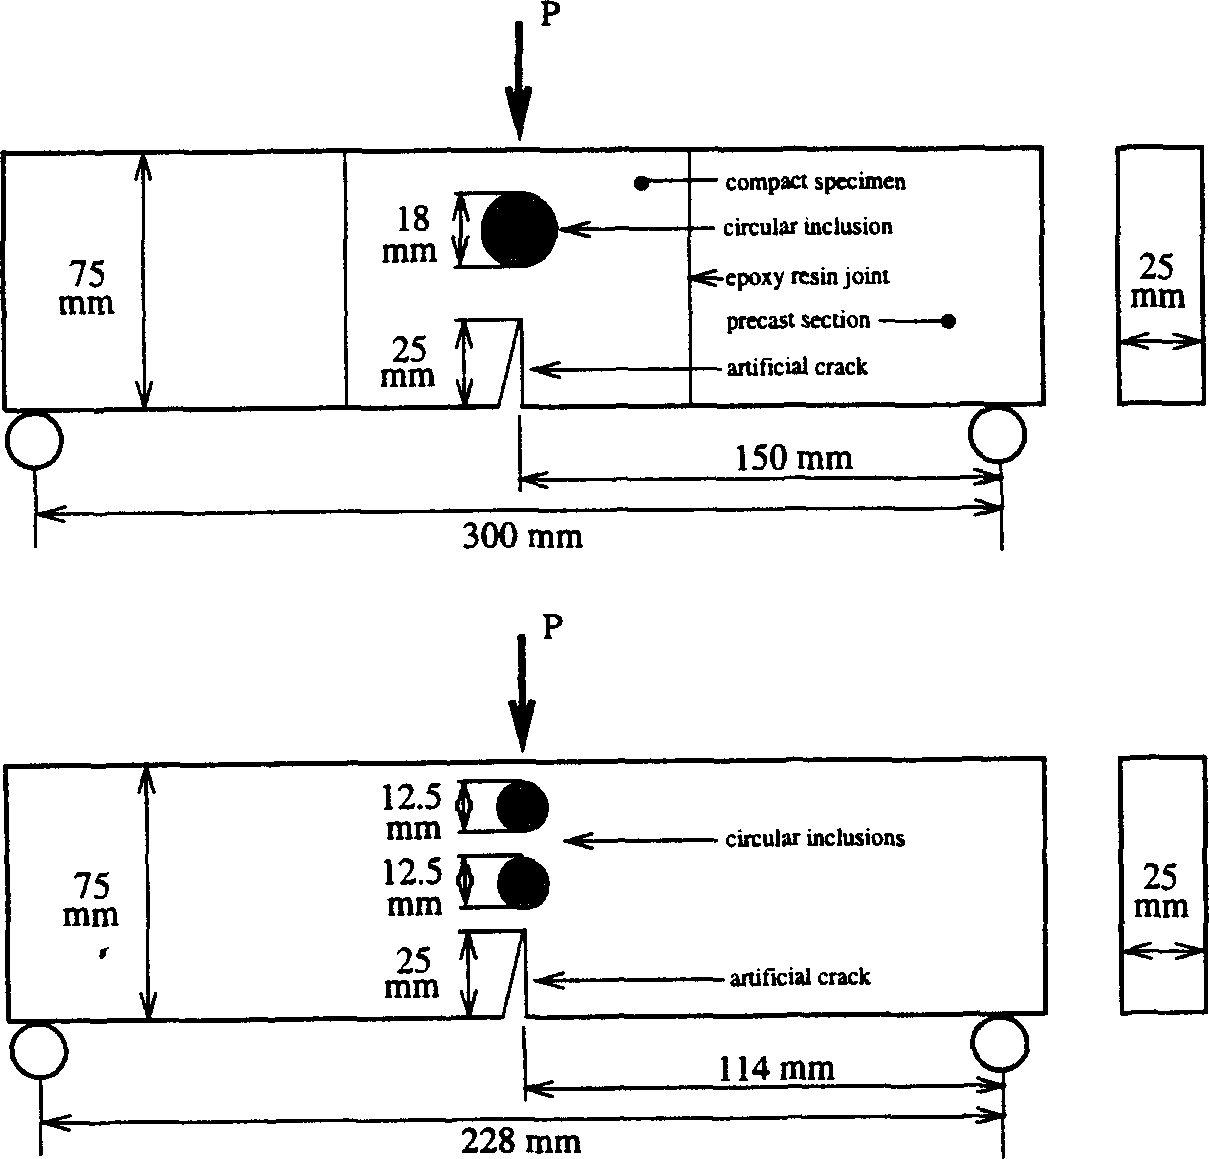
\includegraphics[width=7cm]{mcpm/geomExamples/buyukozturkEtAl}
	\caption[Examples of artificial geometry]{Examples of artificial geometry: \cite{TreggerCorrGrahambradyShah2006a} left and \cite{BuyukozturkHearing1998} right}
	\label{figMCPMLitratureMesoGeometryArtificial}
\end{figure}

The aggregates are modeled as one rigid particle
\cite{%
	GuHongWangLin2013a,%
	WangLinGu2008a,%
	YipLiLiaoBolander2006a,%
	LandisBolander2009a,%
	AsahinaLandisBolander2011a%
} or as a cluster of particles/elements (e.g., spheres in DEM), see figure \ref{figMCPMClusters}
\cite{%
	AzevedoLemosAlmeida2008a,%
	GrasslJirasek2010a,%
	GrasslRempling2008a,%
	GrohKonietzkyWalterHerbst2011a,%
	KimAlrub2011a,%
	PanFengJinXuSunZhangOwen2013a,%
	QinZhang2011a%
}.
Such clustered particles may be rigid or deformable.
\begin{figure}%[htb]
	\centering
	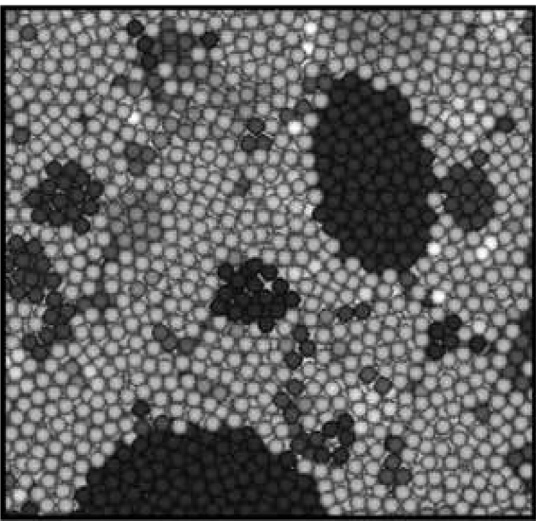
\includegraphics[width=3cm]{mcpm/geomExamples/grohEtAl}
	\hspace{5mm}
	\includegraphics[width=6cm]{mcpm/geomExamples/qinEtAl}
	\hspace{5mm}
	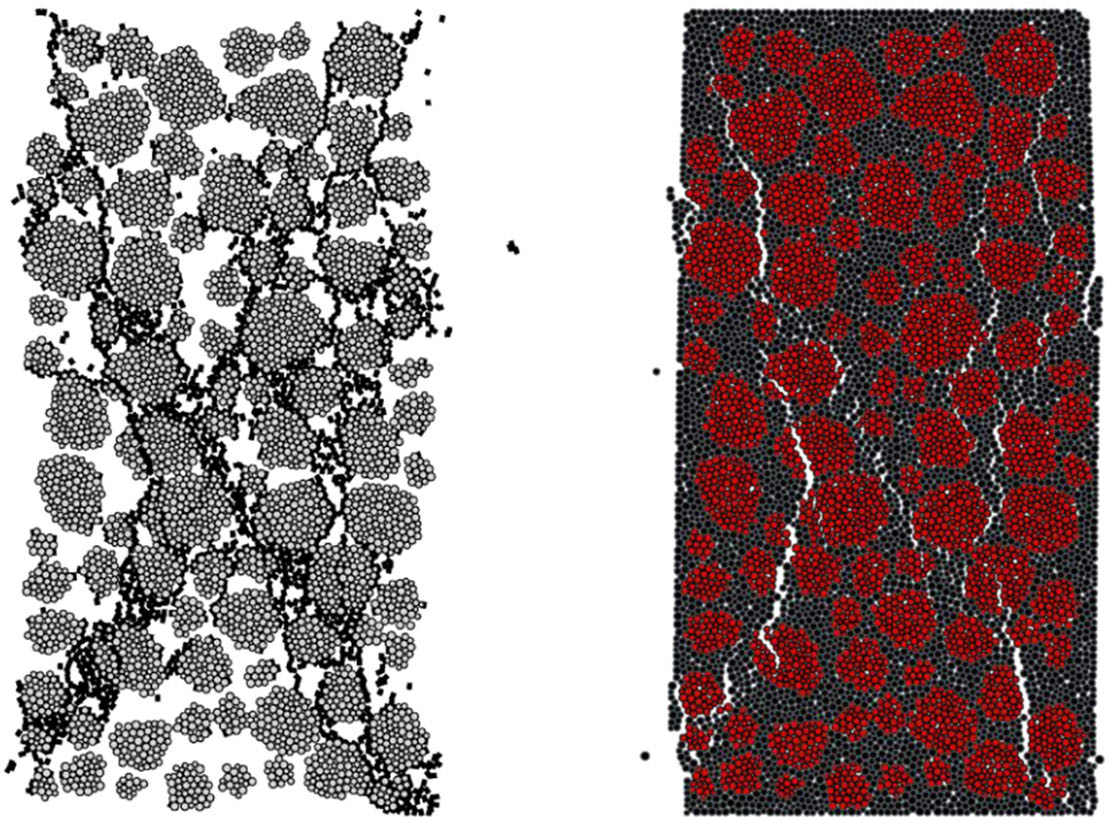
\includegraphics[width=4cm]{mcpm/geomExamples/panEtAl}
	\caption[Illustration of aggregate representation as a cluster of DEM particles]{
		Illustration of aggregate representation as a cluster of DEM particles:
		\cite{GrohKonietzkyWalterHerbst2011a} (left),
		\cite{QinZhang2011a} (middle)
		and
		\cite{PanFengJinXuSunZhangOwen2013a} (right)
	}
	\label{figMCPMClusters}
\end{figure}

\section{Material models for mortar and aggregates}
For practical and computational reasons, both matrix and individual aggregates are modeled as homogeneous components.
Some authors (e.g.,
\cite{%
	CaballeroWillamCarol2008a,%
	CombypeyrotBernardBouchardBayGarciadiaz2009a,%
	Cusatis2001a,%
	GhoshChaudhuri2013a,%
	GrasslJirasek2010a,%
	GrasslRempling2008a,%
	GuHongWangLin2013a%
})
consider aggregates as non damageable, so cracks and damage can only propagate in the matrix.
This assumption is reasonable for certain loading scenarios, but is not applicable in a general case, where cracks can propagate also through aggregates (e.g., for light-weight concrete or for dynamic loading).

Although all three phases of concrete composite material may be modeled with different material models
\cite{%
	ZhouHao2008a,%
	ZhouHao2009a%
}, many authors use for matrix, aggregates and ITZ the same material model
\cite{%
	AzevedoLemosAlmeida2008a,%
	GrohKonietzkyWalterHerbst2011a,%
	GuHongWangLin2013a,%
	KimAlrub2011a,%
	MunguleRaghuprasad2011a,%
	PanFengJinXuSunZhangOwen2013a,%
	SatohYamadaIshiyama2013a,%
	WangLinGu2008a,%
	YipLiLiaoBolander2006a,%
	ZhouHao2008b%
}.

In the case of continuous (FEM) models, the material model for matrix and aggregates is usually based on damage-plasticity models.
\begin{figure}[ht]
	\centering
	\includegraphics[width=5cm]{mcpm/modelExamples/caballeroEtAl}
	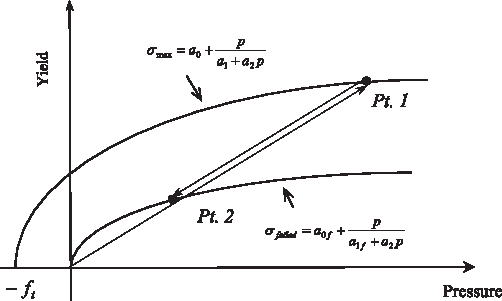
\includegraphics[width=5cm]{mcpm/modelExamples/xuHaoLi}
	\caption[Interface model]{Interface model according to
		\cite{CaballeroWillamCarol2008a} (left)
		and
		\cite{XuHaoLi2012a} (right)
	}
\end{figure}

The discrete models usually work with a more or less complex contact law and a link failure envelope.
See, e.g.,
\cite{%
	CusatisBazantCedolin2006a,%
	GuHongWangLin2013a,%
	IbrahimbegovicDelaplace2003a,%
	QinZhang2011a,%
	TranDonzeMarin2011a,%
	WangLinGu2008a%
} or figure \ref{figMCPMDemModels}.
\begin{figure}[ht]
	\centering
	\newcommand{\hhhh}{\hspace{5mm}}
	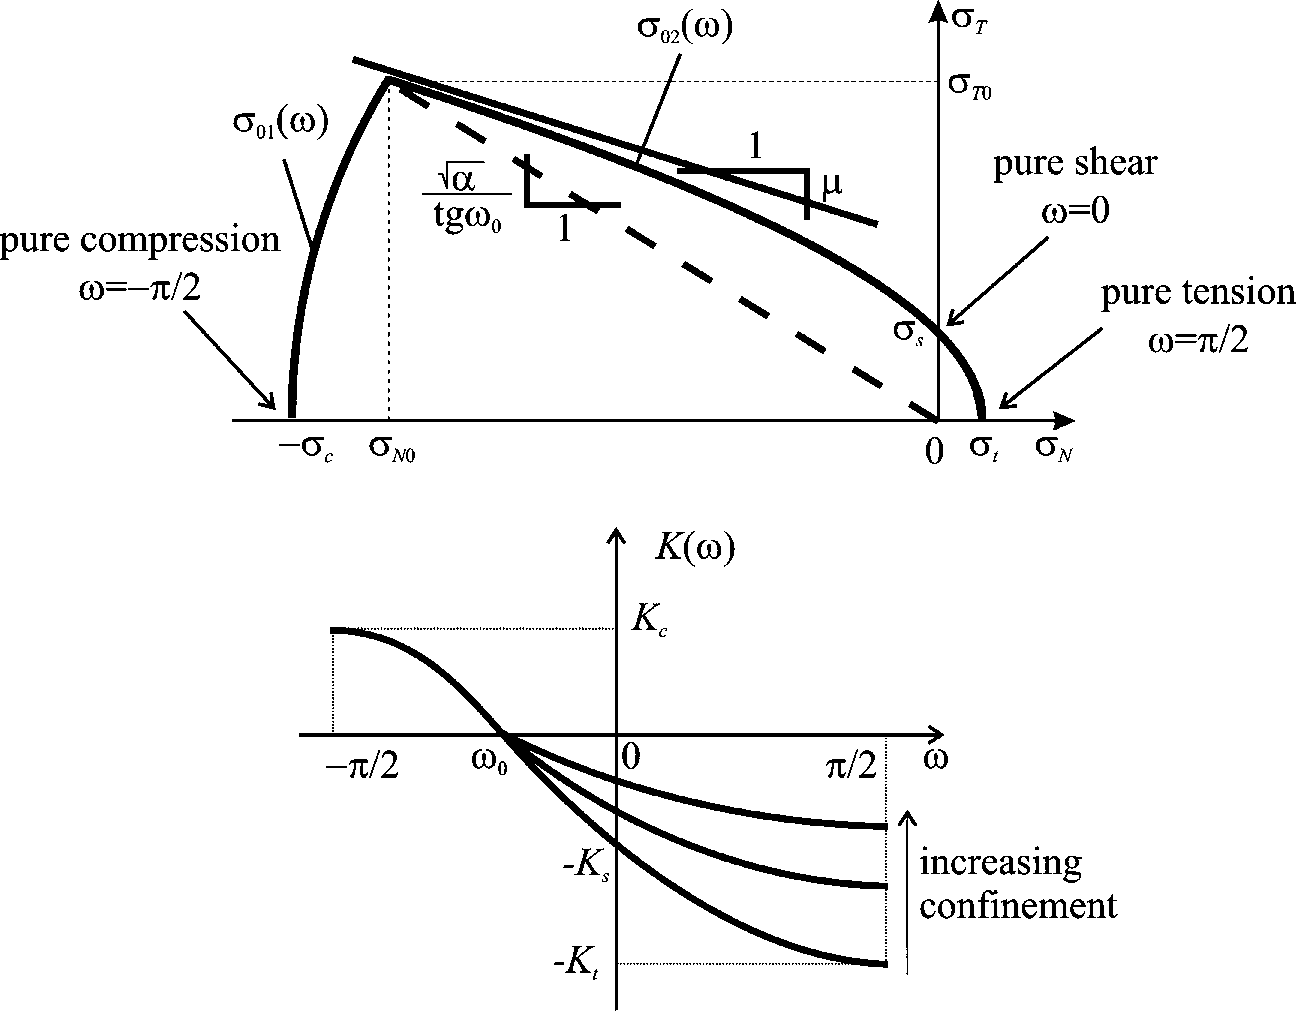
\includegraphics[width=4cm]{mcpm/modelExamples/cusatisEtAl}
	\hhhh
	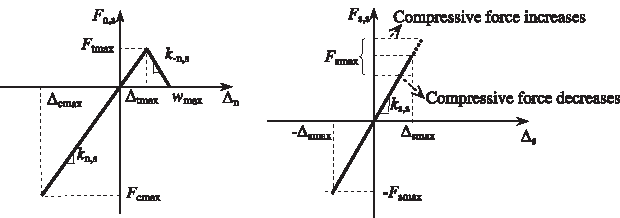
\includegraphics[width=5cm]{mcpm/modelExamples/guEtAl}
	\hhhh
	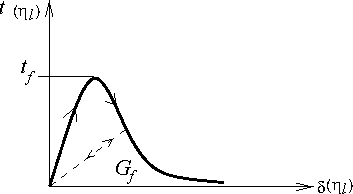
\includegraphics[width=4cm]{mcpm/modelExamples/ibrahimbegovicEtAl}
	\par
	\vspace{5mm}
	\includegraphics[width=5cm]{mcpm/modelExamples/qinEtAl}
	\hhhh
	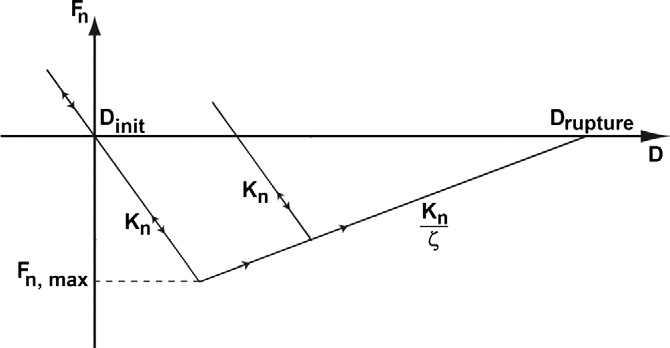
\includegraphics[width=2.5cm]{mcpm/modelExamples/tranEtAl_1}
	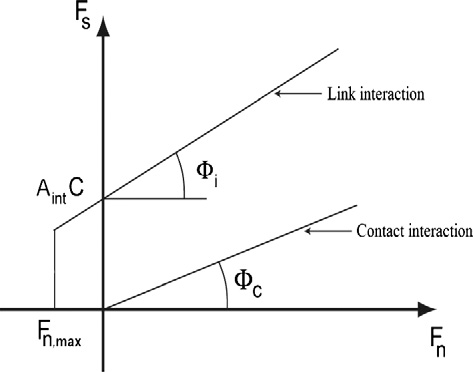
\includegraphics[width=2.5cm]{mcpm/modelExamples/tranEtAl_2}
	\hhhh
	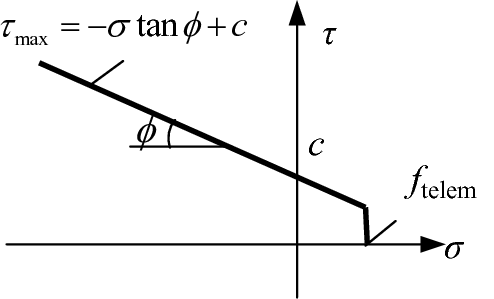
\includegraphics[width=3cm]{mcpm/modelExamples/wangEtAl}
	\caption[Illustration of material models]{Illustration of material models according to
		\cite{CusatisBazantCedolin2006a} (top left),
		\cite{GuHongWangLin2013a} (top middle),
		\cite{IbrahimbegovicDelaplace2003a} (top right),
		\cite{QinZhang2011a} (bottom left),
		\cite{TranDonzeMarin2011a} (bottom middle)
		and
		\cite{WangLinGu2008a} (bottom right)
	}
	\label{figMCPMDemModels}
\end{figure}

Several rock material models (usable for aggregate description) are published in the literature
\cite{
	ErgenzingerSeifriedEberhard2012a,%
	HuangLecampionDetournay2013a,%
	ChoMartinSego2007a,%
	NardinSchrefler2004a,%
	PotyondyCundall2004a,%
	RojekOnateCarlosKargl2011a,%
	ScholtesDonze2013a,%
	ScholtesDonze2012a,%
	TangXuaKoucLindqvistcLiu2001a,%
	WangTonon2009a%
}.
Some of them (see, e.g.,
\cite {
	NardinSchrefler2004a,%
	ScholtesDonze2013a,%
	ScholtesDonze2012a%
} or figure \ref{figMCPMRockModels}) are quite similar to the models of concrete or mortar.
\begin{figure}[ht]
	\centering
	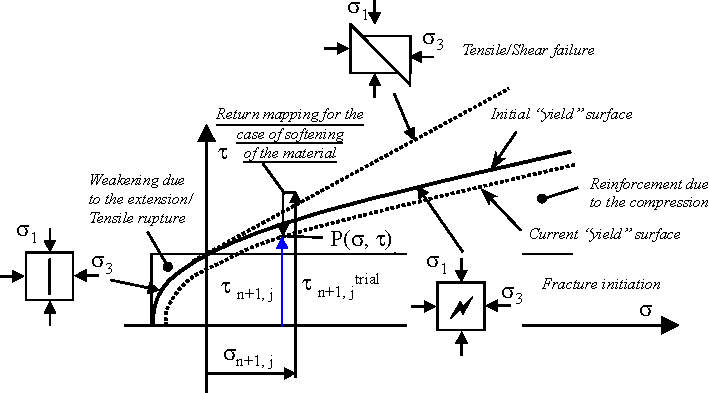
\includegraphics[width=8cm]{mcpm/modelExamples/nardinEtAl}
	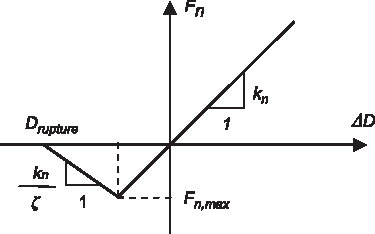
\includegraphics[width=6cm]{mcpm/modelExamples/scholtesEtAl}
	\caption[Illustration of constitutive law]{Illustration of constitutive law according to
		\cite{NardinSchrefler2004a} (left),
		and
		\cite{ScholtesDonze2013a} (right)
	}
	\label{figMCPMRockModels}
\end{figure}

\section{Interface transition zone}
Apart from separated matrix and aggregates, the interface between these components needs to be properly specified for realistic modeling of inelastic processes (crack initiation and propagation for instance).
The interface is a very special region of concrete, occupying a minimal volume, but having a significant influence on resulting concrete properties.

The special role of ITZ is given by both mechanical and chemical reasons, being investigated mathematically and experimentally
\cite{%
	ErdemDawsonThom2012a,%
	GiaccioZerbino1998a,%
	GiaccioZerbinoPonceBatic2008a,%
	RaoPrasad2002a%
}.

From the simulation point of view, the ITZ is often described by the same type of material model as the other constituents, but is considered as the weakest part of the concrete composite, which is reflected in the material parameters choice; see figure \ref{figMCPMItzModeledSameAsMortar}.
\begin{figure}[ht]
	\centering
	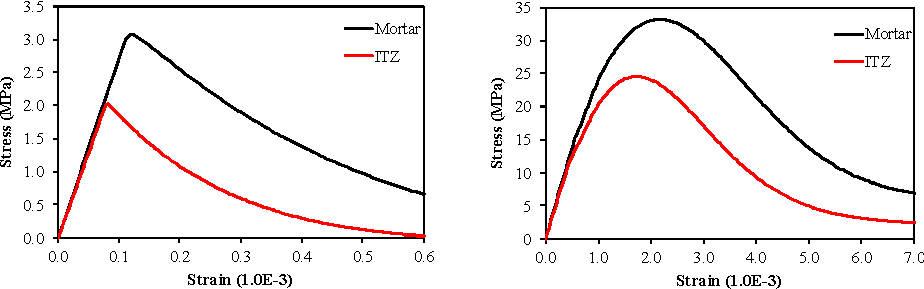
\includegraphics[width=11cm]{mcpm/modelExamples/kimEtAl}
	\caption[ITZ modeled by the same material model]{ITZ modeled by the same material model, only with different parameters
		\cite{KimAlrub2011a}
	}
	\label{figMCPMItzModeledSameAsMortar}
\end{figure}














%%%%%%%%%%%%%%%%%%%%%%%%%%%%%%%%%%%%%%%%%%%%%%%%%%%%%%%%%%%%%%%%%%%%%%
\chapter{New mesoscale discrete element model for concrete}\label{chapMCPMNewModel}
According to the best knowledge of the author, no three-dimensional mesoscale spherical discrete element model for concrete, sufficiently validated against experiments, is published in the literature.
Spherical-like Voronoi diagram based lattice models (e.g.,
\cite{
	CambordeMariottiDonze2000a,%
	Cusatis2001a,%
	GrasslRempling2008a,%
	IbrahimbegovicDelaplace2003a,%
	WangLinGu2008a,%
	YipLiLiaoBolander2006a%
}) might seem to be a solution, but such models do not consider new contacts, the link representation is different from classical spherical discrete elements, etc.
As a~consequence, a new model is proposed.




\section{New model definition}

According to the presented literature study, the author's experience and available simulation tools, the new mesoscale concrete particle model (MCPM) development is summarized in this section.

The discrete element method, using open-source software YADE, is used as a numerical simulation tool.

The material model considered is the CPM, summarized in section \ref{secDemCpm}.
The model considers concrete as a three-phase composite composed of cement paste/mortar matrix, (disordered) aggregates and interfacial transition zone (ITZ) between matrix and aggregates.
The same material model (with different parameters) is considered for all the constituents.

The presented approach considers two types of DEM particles - particles belonging to aggregates and particles belonging to cement mortar.
As a consequence, 3 types of links are possible: aggregate-aggregate, mortar-mortar and aggregate-mortar.
The aggregate-mortar type of links will be called interface links in this thesis.
The material of particles is determined according to the center and size of the particle and according to the geometrical representation (size, shape and orientation) of aggregates.
Figure \ref{figMCPMItzPossibilities} illustrates the approach.
\begin{figure}[htbp]
	\centering
	\includegraphics[width=7cm]{raphaelpy/mcpm_itz_possibilities_1}
	\hspace{2em}
	\includegraphics[width=7cm]{raphaelpy/mcpm_itz_possibilities_2}
	\caption[Illustration of MCPM geometry definition]{Illustration of MCPM geometry definition. Light particles correspond to mortar, dark particles to aggregates and thick links to interface}
	\label{figMCPMItzPossibilities}
\end{figure}

The material models for all constituents (mortar, aggregates, and ITZ) is modeled by the Concrete Particle Model \cite{Smilauer2010a}.
The same model for individual phases is usual among other authors, see section \ref{chapMCPMStateOfTheArt}.

The material properties are constant within mortar and single aggregates (but different aggregates may have different parameters, e.g., simulating concrete with several different aggregate types).
Using this approach, no parts of material are considered as rigid and every part of material may exhibit nonlinear behavior (i.e., aggregates will be deformable and damageable), see figure \ref{figMCPMClusteredAggregateIllustration} for illustration.
\begin{figure}[ht]
	\centering
	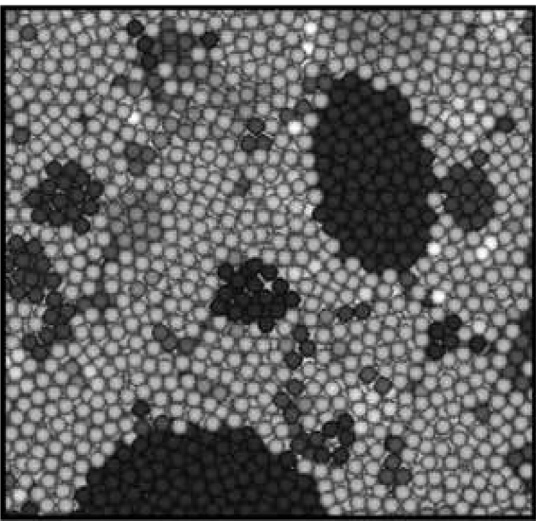
\includegraphics[width=6cm]{mcpm/geomExamples/grohEtAl}
	\caption[Illustration of clustered aggregate]{Illustration of clustered aggregate according to \cite{GrohKonietzkyWalterHerbst2011a}. Different shades indicates different materials}
	\label{figMCPMClusteredAggregateIllustration}
\end{figure}

In YADE default implementation, parameters of links connecting particles with different materials are averaged.
The newly implemented algorithm sets parameters of interfacial links based on the matrix material, with further possibility of stiffness, strength and characteristic length modification.

Numerical studies of other authors \cite{AzevedoLemosAlmeida2008a,KimAlrub2011a,Kozicki2007a,KwanWangChan1999b,GrasslRempling2008a,GuHongWangLin2013a,GrasslJirasek2010a,PradoMier2003a,QinZhang2011a,SnozziGatuingtMolinari2012a,TangZhangShi2008,TreggerCorrGrahambradyShah2006a,YipLiLiaoBolander2006a} consider the interface less stiff and weaker than matrix, see figure \ref{figMCPMITZModelInLiterature}.
This phenomenon is also supported experimentally \cite{TangZhangShi2008}.

\begin{figure}[htbp]
	\centering
	\inputplot{mesoscaleParams}
	\\
	\inputplot{mesoscaleParams_legend}
	\caption[ITZ models in literature]{ITZ models in literature \cite{AzevedoLemosAlmeida2008a,KimAlrub2011a,Kozicki2007a,KwanWangChan1999b,GrasslRempling2008a,GuHongWangLin2013a,GrasslJirasek2010a,PradoMier2003a,QinZhang2011a,SnozziGatuingtMolinari2012a,TangZhangShi2008,TreggerCorrGrahambradyShah2006a,YipLiLiaoBolander2006a}}
	\label{figMCPMITZModelInLiterature}
\end{figure}


For computational reasons, spherical DEM particles with uniform size are used as discrete elements.
The concept of interaction ratio is used in the beginning of the simulation to create cohesive links between mortar-mortar, aggregate-aggregate and mortar-aggregate particles, the latter representing ITZ.









\section{Model validation}

To validate the model for mesoscale concrete, the model should use one set of parameters and should be compared with a set of experiments.
The experimental data of mechanical properties dependent on different aggregate grading curves were chosen for this purpose.

In the literature, there are some studies on this topic, but not all of them suit our purpose.
Some investigate different grading curves, but the aggregates are artificially made, with lower stiffness and strength than the matrix \cite{ElicesRocco2008a}.
Some studies investigate concrete containing a single spherical steel aggregate \cite{AkcaogluTokyayCelik2002a,AkcaogluTokyayCelik2004a,AkcaogluTokyayCelik2005a}.
Others have incomplete input data (e.g, the experiment was intended for a different purpose than we want) \cite{GiaccioZerbino1998a,GiaccioZerbinoPonceBatic2008a}.

The papers are useful anyway providing references to other articles and also summarizing literature research.
Figure \ref{figMCPMValidationFracEnergyOnMaxAggregSize} shows increasing fracture energy for increasing maximum aggregate size \cite{BeygiEtAl2014b}.
Figure \ref{figMCPMValidationMaxAggregSizeInfluenceElicesRocco} shows influence of maximum aggregate size on various concrete mechanical properties \cite{ElicesRocco2008a}.
Black arrows indicate increase, gray dashed arrows decrease and thick gray lines approximately no change.
For increasing maximum aggregate size, fracture energy $G_f$ always increased, but for other quantities ($f_t$ and $E$), the trend is not so indubitable.

\begin{figure}[htbp]
	\centering
	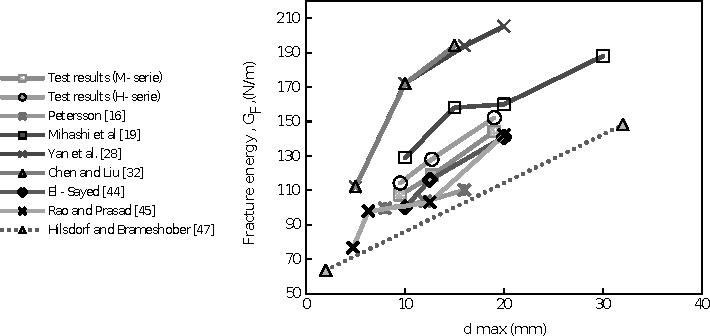
\includegraphics[width=13cm]{mcpm/validation/beigyEtAl2014_bw}
	\caption[Influence of maximum aggregate size on fracture energy]{Influence of maximum aggregate size on fracture energy \cite{BeygiEtAl2014b}}
	\label{figMCPMValidationFracEnergyOnMaxAggregSize}
\end{figure}

\begin{figure}[htbp]
	\centering
	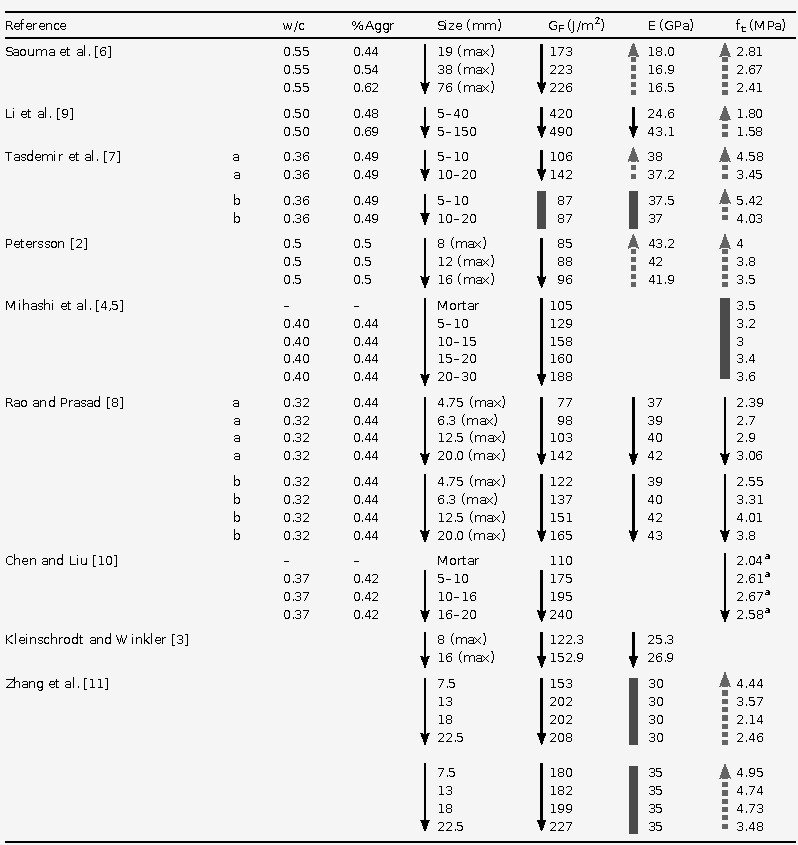
\includegraphics[width=15cm]{mcpm/validation/elicesRocco2008}
	\caption[Influence of maximum aggregate size on mechanical properties]{Influence of maximum aggregate size on mechanical properties \cite{ElicesRocco2008a}}
	\label{figMCPMValidationMaxAggregSizeInfluenceElicesRocco}
\end{figure}



\begin{table}[htbp]
	\centering
	\caption[Concrete compositions]{Cement and water content for concrete compositions [kg/m$^3$] (top) and grading curves [kg/m$^3$] (bottom). The first row of the lower table refers to maximum aggregate size}
	\begin{tabular}{|c|c|c|}
		\hline
		 & $c$ & $w$ \\
		\hline\hline
		low strength  & 325{.}8 & 187{.}0 \\
		\hline
		high strength & 422{.}4 & 160{.}7 \\
		\hline
	\end{tabular}
	\\
	\vspace{1em}
	\begin{tabular}{|rcl|c|c|c|}
		\hline
		     &   &         & 9{.}5 mm & 12{.}5 mm & 19{.}0 mm \\
		\hline\hline
		\multicolumn{3}{|c|}{limestone powder} & 205 & 205 & 205 \\
		\hline
		\multicolumn{3}{|c|}{sand} & 917 & 917 & 917 \\
		\hline
		4.75 & - & 9.5 mm  & 750      & 300       & 300 \\
		\hline
		9.5  & - & 12.5 mm &  -       & 450       & 300 \\
		\hline
		12.5 & - & 19.0 mm &  -       &  -        & 150 \\
		\hline
	\end{tabular}
	\label{tabMCPMValidationBeygiExperiment}
\end{table}

\subsection{Experiment \cite{BeygiEtAl2014a,BeygiEtAl2014b,NikbinEtAl2014a}}

From the studied literature, the experiment from \cite{BeygiEtAl2014a,BeygiEtAl2014b,NikbinEtAl2014a} was chosen.
The experiments investigate the influence of different aggregate sizes (different grading curves) on concrete material properties ($f_t$, $f_c$, $G_f$, $E$).
Two concrete compositions (low strength and high strength) are examined, each with three different aggregate grading curves, see tables \ref{tabMCPMValidationBeygiExperiment}.

Figures \ref{figMCPMValidation} show the comparison between simulations and experimental data.
Since the absolute values of macroscopic quantities can be relatively easily estimated (see section \ref{secDemCpmStructBehavior}), only values relative to the results for the smallest aggregate size are plotted.

Each point in the graphs is the averaged simulation result from 3 runs.
For each run, the same aggregate sizes were considered (according to the corresponding concrete composition and grading curve) and their positions were chosen randomly.
The simulations were performed on 50 mm cubic samples with 2 mm DEM particle size (diameter).
If particles should be considered as mortar or aggregate particles (and consequently identifying ITZ links) was determined according to figure \ref{figMCPMItzPossibilities}

Several combinations of input parameters were tested. The results are plotted for
aggregates 2.5 time stiffer and 5 time stronger than matrix
and for
ITZ 2 times less stif and 2 times weaker than mortar links.
Results 2 refer to 2 times more brittle ITZ than results 1.

The model results reasonably correspond to the trends observed in the experiments, although the precise values are fitted with a certain discrepancy.



\begin{figure}[htbp]
	\centering
	\inputplot{validationBeygi_l}
	\inputplot{validationBeygi_h}
	\caption[Comparison of simulations and experiment]{Comparison of simulations and experiment \cite{BeygiEtAl2014a,BeygiEtAl2014b,NikbinEtAl2014a} for low strength (top) and high strength (bottom) concrete.}
	\label{figMCPMValidation}
\end{figure}
